\documentclass[letterpaper,11pt]{article}

\usepackage{geometry}
\usepackage{pslatex}
\usepackage{fancyhdr}
\usepackage{graphicx}
\usepackage{color}
\usepackage{enumitem} % for ordered list labels
\usepackage{amssymb} % for symbols
\usepackage{scrextend} % for indentation
\usepackage{tabto} % for tabs
\usepackage{amsmath} % for text in equation
\usepackage{forest, tikz} % to make forest

\graphicspath{ {./} }
\geometry{ margin = 1.0in }

%%% TODO modify these variables %%%
\def\homeworknum{6}
\def\myname{Harshit Jain}
\def\myaccessid{hmj5262}
\def\myrecitation{8}
%%%%

\pagestyle{fancy}
\lhead{{\bf CMPSC 465 Fall 2022}}
\chead{{\bf Assignment~\homeworknum}}
\rhead{{\bf \today}}

\newcounter{problemid}
%\stepcounter{problemid}
\def\newproblem{\clearpage\newpage{\bf Problem~\arabic{problemid}\stepcounter{problemid}}\hfill\fbox{\parbox{0.16\textwidth}{\bf Points:}}\par}

\setlength\parindent{0em}
\setlength\parskip{8pt}
\setlength{\fboxsep}{6pt}


\begin{document}

\framebox[\textwidth]{
	\parbox{0.96\textwidth}{
		\parbox{0.12\textwidth}{\bf Name:}\parbox{0.6\textwidth}{\myname}\\
		\parbox{0.12\textwidth}{\bf Access ID:}\parbox{0.6\textwidth}{\myaccessid}\\
		\parbox{0.12\textwidth}{\bf Recitation:}\parbox{0.6\textwidth}{\myrecitation}
	}
}


%% your solutions %%%

\newproblem
\textbf{Acknowledgements}
\begin{enumerate}[label=(\alph*)]
    \item I did not work in a group.
    \item I did not consult without anyone my group members.
    \item I did not consult any non-class materials.
\end{enumerate}


% PROBLEM 1
\newproblem
\textbf{DFS variations}
\begin{enumerate}[label=(\alph*)]
    
    \item 
    \textbf{Algorthm:} It is given that the car can only hold enough gas to cover $L$ miles while any stretch of highway $(l_e)$ $e \in E$ may or may not
    be greater than $L$. Therefore, initially we can simply remove edges $(e)$ of a greater value.
    Now, the next step is to see if the city $t$ is still reachable from $s$. To check that, we will be using Breadth First Search $(BFS)$ algorithm.
    So if vertex $t$ is reachable, then the path is feasible otherwise, it is not feasable.
    
    % \textbf{Proof:} In order to show correctness of the algorithm, we would have to show two things:
    % \tabto{30pt}(1) If a solution exists, the algorithm will find it
    % \tabto{30pt}(2) If the algorithm finds a solution, then it’s a valid solution
    

    % \tabto{30pt} \underline{Base Case:}

    % \tabto{30pt} \underline{Inductive Step:} 
    
    \textbf{Runtime:} Running $BFS$ will take $O(|V|+|E|)$.


    
    \item Here, we will modify Dijkstra's algorithm to find paths that minimize the maximum weight of any edge on the path
    (instead of the path length).
    
    Here, we take minimum of max$($visited, not visited adjacent$)$.

    \textbf{Algorthm:}

    ModifiedDijkstra$(G=(V,E))$
    \tabto{25pt} \textbf{for} all $u \in V$ \textbf{do}
        \tabto{50pt} dist$(u)$ = $\infty$
        \tabto{50pt} prev$(u)$ = nil
    \tabto{25pt} \textbf{end}
    \tabto{25pt} dist$(s)=0$
    \tabto{25pt} Let $H$ be a priority queue constructed with all nodes in $V$ using $dist$ as the key
    \tabto{25pt} \textbf{while} $H$ is not empty \textbf{do}
        \tabto{50pt} $u=$ deleteMin$(H)$
        \tabto{50pt} \textbf{for} all edges $(u,v) \in E$ \textbf{do}
            \tabto{75pt} \textbf{if} dist$(v) >$ max$(\text{dist}(u), \text{l}(u,v))$ \textbf{then}
                \tabto{100pt} dist$(v) =$ max$(\text{dist}(u), \text{l}(u,v))$
                \tabto{100pt} prev$(v) = u$
                \tabto{100pt} decreaseKey$(H,v)$
            \tabto{75pt} \textbf{end}
        \tabto{50pt} \textbf{end}
    \tabto{25pt} \textbf{end}
    \tabto{0pt} \textbf{end}
    
    \textbf{Runtime:} Time complexity is same as Dijkstra's algorithm i.e. $O((|V|+|E|)log|E|)$.




\end{enumerate}



% PROBLEM 2
\newproblem
\textbf{Shortest bitonic paths}
\begin{enumerate}[label=(\alph*)]
    
    \item 
    
    \item

\end{enumerate}


% PROBLEM 3
\newproblem
\textbf{Dijkstra’s on negative}
\begin{enumerate}[label=(\alph*)]
    
    \item 
    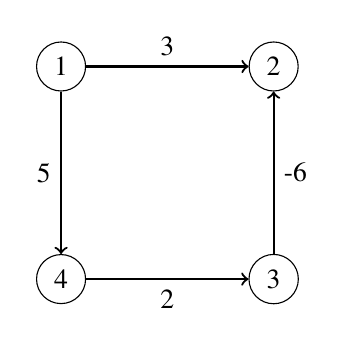
\begin{tikzpicture}[scale=0.9,auto=center]
        \node[circle, draw] (1) at (0, 0) {$1$};
        \node[circle, draw] (2) at (3, 0) {$2$};
        \node[circle, draw] (3) at (3, -3) {$3$};
        \node[circle, draw] (4) at (0, -3) {$4$};

        \draw[->, thick] (1) to node[anchor=south]{3} (2);
        \draw[->, thick] (1) to node[anchor=east]{5} (4);
        \draw[->, thick] (4) to node[anchor=north]{2} (3);
        \draw[->, thick] (3) to node[anchor=west]{-6} (2);
    \end{tikzpicture}
    
    Starting node $: 1$

    Here, the Dijkstra's algorithm give the shortest path to node $2$ as $3$ however if we follow along the path $\textbf{1} \rightarrow \textbf{4} \rightarrow \textbf{3} \rightarrow \textbf{2}$,
    we get the shortest path as $(5+2-6) = \textbf{1}$. So, clearly the Dijkstra's algorithm does not produce the correct algorithm.

    \item When the input graph contains negative edges, the following statement from the handout does not necessarily hold:
    
    \begin{itemize}
        \item The $dist$ for values already in $R$ is not modified. 
        \item Also, because $x$ is in $R$, it must have removed from $H$ during a previous iteration and had all its outgoing edges updated.
    \end{itemize}
    The $dist$ for values already in $R$ can still be modified if we encounter a negative edge in a different path which leads to the value already in $R$ and
    results in the shorter path (value) than the one it had previously in $R$. If the edge weight is negative, then adding an edge
    can indeed make the path length shorter and this is where Dijkstra's Algorithm fails.
\end{enumerate}
\end{document} 
